\documentclass{article}

\usepackage[final]{neurips_2019}

\usepackage[utf8]{inputenc}
\usepackage[T1]{fontenc}
\usepackage{hyperref}
\usepackage{url}
\usepackage{booktabs}
\usepackage{amsfonts}
\usepackage{nicefrac}
\usepackage{microtype}
\usepackage{graphicx}
\usepackage{xcolor}
\usepackage{lipsum}
\usepackage{listings}
\usepackage{tikz}
\usepackage{amsmath}
\usepackage{subcaption}
\usepackage{float}
\newcommand{\note}[1]{\textcolor{blue}{{#1}}}
\usetikzlibrary{positioning}

\title{
  Size Doesn't Matter If You Search Enough\\
  \vspace{1em}
  \small{\normalfont Stanford CS224N Custom Project} 
}


\author{
  Yalcin Tur \\
  Department of Computer Science \\
  Stanford University \\
  \texttt{yalcintr@stanford.edu} \\
  % Examples of more authors
\And
   Mihajlo Stojkovic \\
   Department of Computer Science \\
   Stanford University \\
   \texttt{mstojkov@stanford.edu} \\
   \And
   Angel Raychev \\
   Department of Computer Science \\
   Stanford University \\
   \texttt{angelray@stanford.edu}
}
\begin{document}

\maketitle


\begin{abstract}
In this paper, we investigate how smaller-scale language models (135M, 360M, and 1.7B parameters) can achieve superior reasoning performance through extensive Monte Carlo Tree Search (MCTS) inference and iterative synthetic training. Inspired by AlphaZero and recent TS-LLM approaches, we demonstrate that small-scale SmolLM2 models within an explicit MCTS framework can outperform significantly larger models on structured reasoning tasks. Our 135M parameter model achieves 29.4\% accuracy on the Game of 24, surpassing GPT-4o's zero-shot performance (20.6\%). The 360M and 1.7B models reach even higher performance, with 53.4\% and 54.6\% accuracy respectively. Our key contributions include: (1) a systematic evaluation of scaling behaviors across multiple combinations of policy and value model sizes, (2) a novel iterative synthetic training framework that continuously refines model capabilities using automatically generated MCTS trajectories, with each iteration yielding approximately 10\% performance improvement, and (3) empirical evidence showing that substantial inference-time computational investment can effectively mitigate and even overcome the limitations typically associated with smaller model sizes.
\end{abstract}

\section{Key Information}
\begin{itemize}
    \item Mentor: Anjiang Wei and Rafael Rafailov
    \item External Collaborators: N/A
    \item Sharing project: Angel is enrolled in CS234 where he is individually pursuing a project that uses our work here as a baseline and propose a new method for MCTS using dynamic branching.
\end{itemize}


\section{Introduction}
Large Language Models (LLMs) \cite{dubey2024llama, achiam2023gpt, jiang2024mixtral} have demonstrated impressive capabilities in various natural language tasks, but their structured and multi-step reasoning abilities remain limited, particularly when solutions require extensive exploration of possible pathways. Current state-of-the-art reasoning methods rely primarily on increasingly large-scale models and resource-intensive inference processes, often posing substantial computational challenges and practical limitations. Recent advances, such as OpenAI o1 \cite{zhong2024evaluationopenaio1opportunities} and DeepSeek R1 \cite{deepseekai2025deepseekr1incentivizingreasoningcapability}, have demonstrated that sophisticated inference-time methods can notably improve reasoning capabilities without proportional increases in model size.

Nonetheless, established tree-search-based methods—including Tree-of-Thought (ToT) \cite{yao2023tree} and Reasoning via Planning (RAP) \cite{hao2023reasoning}—largely rely on extensive prompt engineering, significant computational overhead from large models, and often limit the search depth to maintain practical inference times. To address these limitations, our research explicitly investigates whether extensive inference-time computational investment using Monte Carlo Tree Search (MCTS) can enable smaller-scale models—specifically, SmolLM2 models of sizes 135M, 360M, and 1.7B parameters—to achieve competitive performance compared to substantially larger models.

We select the Game of 24 as our primary benchmark for several strategic reasons. First, it represents a well-defined mathematical reasoning task that requires both creativity and systematic exploration—players must combine four numbers using basic arithmetic operations to reach exactly 24. Second, its discrete action space and clear evaluation criteria make it ideal for MCTS implementation. Third, the game presents a significant challenge for current LLMs, with even state-of-the-art models like GPT-4o achieving only moderate success rates. Finally, as a task that combines arithmetic reasoning with search space exploration, it serves as an excellent proxy for more complex real-world reasoning problems while remaining tractable for systematic evaluation.

We formulate sentence generation explicitly as discrete actions within an MCTS-driven decision-making framework. Initially, we evaluate nine distinct configurations by independently varying the size of policy and value functions, each trained on synthetic data for one iteration. This allows us to empirically demonstrate scaling behaviors and performance trade-offs clearly. Subsequently, we propose an iterative synthetic training approach, particularly focusing on our smallest model (135M parameters), where policy and value functions are continuously refined through automatically generated, progressively higher-quality MCTS trajectories.

Our key contributions are:

\begin{enumerate}
\item Empirically demonstrating that smaller-scale models (135M, 360M, and 1.7B parameters), when enhanced by extensive MCTS inference, can achieve and surpass the performance of substantially larger models on structured reasoning tasks like the Game of 24, with our smallest 135M model reaching 29.4\% accuracy and our 360M model achieving 53.4\% accuracy.
\item Introducing a multi-iteration synthetic training methodology and codebase leveraging MCTS to iteratively generate improved training data, significantly enhancing the reasoning capabilities of small-scale models, with an iteration providing approximately 10\% performance improvement.
\item Conducting systematic analyses to explore and highlight trade-offs between inference-time computation, training-time investment, branching factors, and exploration counts, addressing a critical gap by providing clear empirical insights into optimal resource allocation.
\end{enumerate}

By addressing the current absence of clear scaling laws and explicitly examining critical trade-offs, our results advocate for a paradigm shift in language model scaling strategies, emphasizing inference-time computational investment over model parameter expansion.

\section{Related Work} Several recent studies have explored methods to augment the reasoning and generation capabilities of LLMs using structured search and planning strategies. Among the earliest is the Tree-of-Thought (ToT) methodology \cite{yao2023tree}, which significantly enhanced LLM reasoning by explicitly exploring alternative reasoning paths within a structured search tree. Similarly, Reasoning via Planning (RAP) \cite{hao2023reasoning} employed MCTS within a world-model framework, using the language model itself to simulate future states and guide reasoning paths with explicit rewards.

The AlphaZero framework \cite{silver2017mastering}, originally developed for game-playing AI, has inspired significant innovation in applying reinforcement-learning-guided tree search to language modeling. The TS-LLM approach \cite{feng2023alphazero} successfully adapted this methodology by using learned policy and value functions within an MCTS framework to guide language model decoding and iterative training. This marked a substantial improvement over purely prompt-based evaluation methods, enabling deeper exploration (up to 64 steps), and provided empirical evidence that coupling inference-time search with learned evaluators considerably improves performance in complex tasks.

Further developments, such as Ensembling LLMs with MCTS \cite{park2024ensemble}, Monte Carlo Tree Self-Refine \cite{zhang2024accessing}, and MCTS-guided code generation methods \cite{dainese2024generating}, underscore the versatility and effectiveness of MCTS in structured and multi-step reasoning scenarios. These studies collectively illustrate that structured search not only enhances LLM performance but also reduces reliance on increasingly large model sizes by focusing computational resources effectively during inference.

\section{Approach}
In this work, we implement Monte Carlo Tree Search, inspired by AlphaZero \cite{silver2017mastering}, to address the Game of 24 within the language model domain. We analyze scaling laws related to training compute, test compute, policy model size, and value model size. Our methodology primarily follows the TS-LLM framework introduced in \cite{feng2023alphazero}. The details of our approach are outlined in the following section.


\subsection{Background}
We frame the language model's generation process within a reinforcement learning context, explicitly defining states and actions. Each generated sentence represents an action, and the state comprises the sequence of sentences generated thus far. Formally, given an input question \(q\) and generated sentences \(a_1, a_2, \ldots, a_T\), the initial state is \(s_0 = q\), and subsequent states are defined as \(s_t = q a_1 a_2 \ldots a_t\).

We introduce an oracle reward function \(r: \mathcal{A} \rightarrow \{0, 1\}\), assigning a reward of 1 for correct final solutions and 0 otherwise. Intermediate rewards are disregarded, so the reward is evaluated only at the terminal state. Consequently, the reward for trajectory \(\tau = q a_1 a_2 \ldots a_T\) is \(r(a_T)\).

Our language model \(\pi_\theta\) generates probability distributions over the token dictionary, effectively functioning as a stochastic policy. Specifically, \(\pi_\theta(a_t \mid s_{t-1})\) denotes the probability of generating sentence \(a_t\) given state \(s_{t-1}\).

Following the RL paradigm, we define a value function \(v(s)\) representing the expected reward when starting from state \(s\) and following policy \(\pi_\theta\). Given that our reward is binary and evaluated only at the terminal state, \(v(s)\) directly corresponds to the probability of achieving a correct solution from state \(s\). Inspired by the AlphaZero framework, we approximate \(v(s)\) using a learned model \(v_\phi(s)\).

\subsection{Monte Carlo Tree Search (MCTS)}
MCTS iteratively performs four stages: selection, expansion, evaluation, and backpropagation. In the selection phase, actions are chosen using an upper confidence bound:
$$
a = \arg\max_{a \in \mathcal{A}} \left(Q(s,a) + c \cdot \frac{\sqrt{N(s)}}{N(s,a) + 1}\right),
$$
where \(Q(s,a)\) is the average backpropagated value for action \(a\) taken from state \(s\), \(N(s)\) is the visit count for state \(s\), \(N(s,a)\) is the count of action \(a\) selected from state \(s\), and \(c\) is an exploration constant balancing exploitation and exploration. Selection continues until reaching a leaf node or a terminal state. Upon reaching a leaf node \(s_{\text{leaf}}\), we expand the node by generating \(b\) actions using the policy \(\pi_\theta\):
$$
a_1, a_2, \ldots, a_b \sim \pi_\theta(\cdot \mid s_{\text{leaf}}).
$$
Each generated action is evaluated using the value function \(v_\phi\):
$$
v_\phi(s_{\text{leaf}}, a_k), \quad k=1, \ldots, b.
$$
We initialize \(N(s_{\text{leaf}},a_k) = 0\) and set \(Q(s_{\text{leaf}},a_k) = v_{\phi}(s_{\text{leaf}},a_k)\), then proceed to backpropagation. If a terminal state is reached, expansion and evaluation are skipped, and we directly proceed to backpropagation. During backpropagation, we traverse from \(s_{\text{leaf}}\) back to the root, incrementing visit counts \(N(s)\) and \(N(s,a)\) and updating \(Q(s,a)\) as:
$$
Q(s,a) \leftarrow Q(s,a) + \frac{1}{N(s,a)} \left(v_{\phi}(s_{\text{leaf}}) - Q(s,a)\right).
$$
MCTS terminates once some predefined condition is met. For example, we have made a certain number of expansions, or we have reached a certain number of leaves, or the visit count of the root has exceeding a certain limit.

\subsection{Training}
We use MCTS to generate trajectories that lead to terminal states. Positive trajectories are used to further refine the policy model, with the policy loss defined as:
\[
\mathcal{L}_{\text{policy}} = \mathbb{E}_{q \sim Q_{\text{train}}, s\sim\mathcal{D}_q^+}\Big[-\log \pi_\theta(s)\Big],
\]
where \(q\) is sampled uniformly from the training dataset \(Q_{\text{train}}\), and \(\mathcal{D}_q^+\) denotes the distribution of positive trajectories generated from question \(q\). To train the value function, we use both positive and negative trajectories and minimize a binary classification loss defined as:
\[
\mathcal{L}_{\text{value}} = \mathbb{E}_{q \sim Q_{\text{train}}, s \sim \mathcal{D}_q} \Big[ \ell_{\text{BCE}} (v(s), r(s)) \Big],
\]
where \(\mathcal{D}_q\) is the distribution of both positive and negative trajectories sampled from question \(q\). By continuously generating new trajectories using MCTS and training our models with this freshly gathered data, we iteratively enhance both the policy and the value function.


\subsection{Inference}
For inference, we again utilize MCTS. Given a question $q$, we employ the trained policy and value function to conduct MCTS starting from $q$. The search continues until we exhaust a predefined computational budget, determined by the number of expansions multiplied by the branching factor and the computational cost of generating each action. During inference, we no longer have access to the oracle reward model to directly select a positively evaluated trajectory. After we have finished growing the tree, we start from the root node and iteratively select the action with the highest visitation count $N(s,a)$ at each step until reaching a leaf node. The resulting sequence of actions is then output as our proposed solution.

\section{Implementation Details and Dataset}


\subsection{Dataset Statistics and Data Format}

The training dataset consists of 1,362 unique combinations of four numbers, partitioned into 1,000 training, 100 validation, and 162 test examples. Both the policy and value function models share the same fundamental data structure, comprising a current state (four numbers) accompanied by a sequence of intermediate arithmetic steps (Figures \ref{examle_policy}, \ref{examle_value_function}). The policy model is trained to generate a suitable next action based on the given state, whereas the value function model estimates the probability of successfully reaching a solution from that state.

\begin{figure}[H]
    \centering
    % Left diagram: Chat-based data structure
    \begin{minipage}{0.4\textwidth}
        \centering
        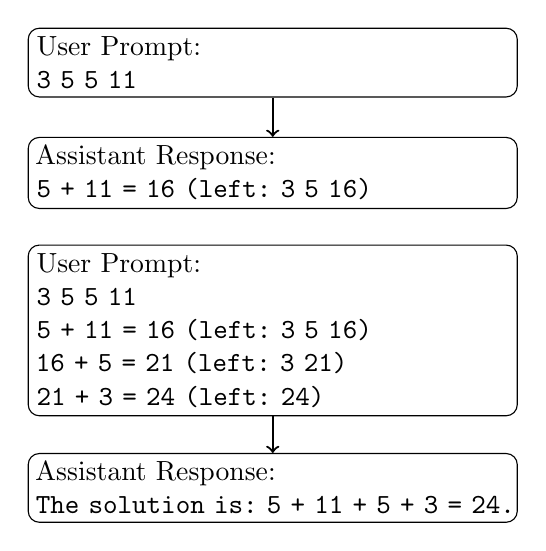
\begin{tikzpicture}[
            node distance=2cm, auto,
            every node/.style={rectangle, draw, rounded corners, text width=6cm, inner sep=3pt}
        ]
            \node (prompt) {User Prompt:\\ \verb|3 5 5 11|};
            \node (response) [below=0.5cm of prompt] {Assistant Response:\\
                \verb|5 + 11 = 16 (left: 3 5 16)|};

            \node (2prompt)  [below of=response] {User Prompt:\\ \verb|3 5 5 11|\\
                \verb|5 + 11 = 16 (left: 3 5 16)|\\
                \verb|16 + 5 = 21 (left: 3 21)|\\
                \verb|21 + 3 = 24 (left: 24)|\\
            
            };
            \node (2response) [below of=2prompt] {Assistant Response:\\
                \verb|The solution is: 5 + 11 + 5 + 3 = 24.|};
            
              node[above=4pt, right=6pt, drawn = none, fill = none] {\small \textbf{Chain-of-Thought}};
            \draw[->, thick] (prompt.south) -- (response.north);
            \draw[->, thick] (2prompt.south) -- (2response.north);
        \end{tikzpicture}
        \caption{Policy Model Input-Output Examples}
        \label{examle_policy}
    \end{minipage}
    \hfill
    % Right diagram: Value function evaluation structure
    \begin{minipage}{0.48\textwidth}
        \centering
        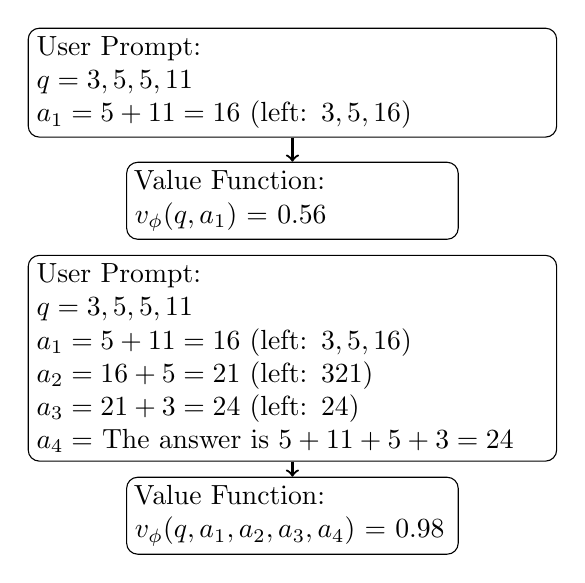
\begin{tikzpicture}[
            node distance=2cm, auto,
            every node/.style={rectangle, draw, rounded corners, text width=6.5cm, inner sep=3pt}
        ]
            \node (q) {User Prompt:\\ $q = 3, 5, 5, 11$ \\
            $a_1 = 5 + 11 = 16$ (left: $3, 5, 16$) \\ 
            };
        
            \node (vf) [below of=q, node distance=1.5cm, text width=4cm] {Value Function:\\ $v_\phi(q, a_1)$ = 0.56};

           \draw[->, thick] (q.south) -- (vf.north);

           
            \node (2q) [below of=vf]{User Prompt:\\ $q = 3, 5, 5, 11$ \\
            $a_1 = 5 + 11 = 16$ (left: $3, 5, 16$) \\ 
            $a_2 = 16 + 5 = 21$ (left: $3 21$)\\
            $a_3 = 21 + 3 = 24$ (left: $24$)\\
            $a_4 =$  The answer is $5 + 11 + 5 + 3 = 24$
            };
        
            \node (2vf) [below of=2q, node distance=2cm, text width=4cm] {Value Function:\\ $v_\phi(q, a_1, a_2, a_3, a_4)$ = 0.98};
            \draw[->, thick] (2q.south) -- (2vf.north);

           
        \end{tikzpicture}
        \caption{Value Model Input-Output Examples}
        \label{examle_value_function}
    \end{minipage}
\end{figure}

\subsection{Iterative Policy and Value Model Training via MCTS}

We use the SmolLM2 models \cite{allal2025smollm2} for both the policy model $\pi_\theta$ and the value model $v_\phi$. The policy is initialized by fine-tuning the Instruct variant on a synthesized dataset to enforce correct output formatting (see Figure \ref{examle_policy}). For the value function, we adapt the Base variant by replacing the final \textbf{Linear $\to$ Softmax} layer—which typically maps hidden representations to vocabulary logits—with a dedicated value head composed of a \textbf{Linear $\to$ ReLU $\to$ Linear $\to$ Sigmoid} sequence (Figure \ref{value_function_architecture}), following guidance from the TS-LLM architecture proposed in \cite{feng2023alphazero}.

Training data for both models is generated via Monte Carlo Tree Search. At each iteration, we gather 40 terminal trajectories per problem instance using the current policy and value function. Positive trajectories are utilized for further policy fine-tuning, while both positive and negative trajectories are used for the training of the value function via binary cross-entropy loss. After each training phase, updated models are deployed to inference servers for data generation in subsequent iterations.

During MCTS data generation, we employ the following hyperparameters: branching factor $b = 3$, a maximum of 20 node expansions per search tree, and an exploration constant $c = 0.3$. An ablation study (Table \ref{tab:temperature-analysis}) determined the optimal temperature parameter to be $t=1$ (see Appendix). For the initial iteration, the policy model is the synthesized-data fine-tuned variant, and the value function is uniformly initialized at 0.5, effectively implementing a breadth-first search.



\begin{figure}[H]
    \centering
    \includegraphics[width=0.9\textwidth]{valfunc.png}  % Adjust width accordingly
    \caption{Illustration of the value function architecture.} 
    \label{value_function_architecture}  
\end{figure}

\subsection{Deployment and Serving Infrastructure}
For inference serving, all models are deployed on RTX 4090 GPUs. The policy models are served using the vLLM library \cite{kwon2023efficient}, achieving the following throughputs: the 135M model processes 120 requests per second (req/s), the 360M model achieves 90 req/s, and the 1.7B model attains 50 req/s.

For serving the value models, we employ a combination of PyTorch and FastAPI, providing throughputs of 70 req/s for the 135M model, 45 req/s for the 360M model, and 30 req/s for the 1.7B model. While vLLM is more efficient, our custom modifications to the value function head necessitated this traditional serving approach. Additionally, policy models are served at full precision, whereas value models utilize half-precision for computational efficiency.

The Hugging Face library (SFTTrainer) \cite{allal2025smollm2} was employed for fine-tuning the policy models and we have written the custom training script for finetuning the value function. The entire project codebase including evaluation, fine-tuning, and data creation was developed by our team.

\subsection{Experimental Details and Evaluation}

We conducted our experiments using SmolLM2 models \cite{allal2025smollm2} with parameter sizes of 135M, 360M, and 1.7B, aiming to explore the interplay between Monte Carlo Tree Search and model performance, particularly focusing on scaling effects for both policy and value functions.

In total, we trained 11 models across multiple iterations, covering different sizes and functions: policy models (135M: iterations 0–2; 360M and 1.7B: iterations 0–1) and value models (135M: iterations 1–2; 360M and 1.7B: iteration 1). Detailed training procedures and inference specifics are described in Section 4, and training hyperparameters for each iteration are available in the Appendix.

We evaluated the performance of our SmolLM2-based methods using the accuracy metric. The accuracy was computed by strictly verifying three essential components of each generated solution: confirming that the final computed value exactly equals 24, ensuring that the arithmetic operations used are valid, structurally coherent, and executable, and verifying that the generated solution strictly uses only the provided numbers without omission or repetition beyond the given frequency.

\section{Results and Analysis}

We present a comprehensive analysis of our MCTS-enhanced small language models across multiple dimensions: baseline performance comparison, scaling behavior with computational resources, iterative improvement through synthetic training, and the impact of search hyperparameters on model performance.

\begin{table}[h]
    \centering
    \caption{Baseline Model Performance on the Game of 24 Task}
    \label{tab:baselines}
    \begin{tabular}{p{2cm}p{3cm}p{3cm}p{3cm}}
        \toprule
        \textbf{Model} & \textbf{Zero-shot (SFT)} & \textbf{Auto-CoT \cite{zhang2022automaticchainthoughtprompting}} & \textbf{ToT \cite{yao2023tree} (n=3)} \\
        \midrule
        135M   & 2.76\%  & 3.02\%  & 9.21\% \\
        360M   & 3.87\%  & 3.94\%  & 14.76\% \\
        1.7B   & 4.97\%  & 7.08\%  & 22.01\% \\
        GPT-4o & 20.60\% & 32.44\% & 45.89\% \\
        \bottomrule
    \end{tabular}
\end{table}

Table \ref{tab:baselines} illustrates the performance of various models on the Game of 24 task without MCTS enhancement. As expected, model performance scales with parameter count across all inference methods. Even with simpler prompting techniques such as zero-shot and Chain-of-Thought (CoT), larger models consistently outperform smaller ones. Tree-of-Thought (ToT) significantly improves performance across all model sizes, demonstrating the value of structured search in reasoning tasks. (ToT (branch factor 3) \cite{yao2023tree} and Auto-CoT \cite{zhang2022automaticchainthoughtprompting} are evaluated with the code in their official repositories.)

GPT-4o (evaluated with the prompt in the Appendix) achieves substantially higher accuracy than all SmolLM2 variants across each inference method, establishing a strong upper bound for comparison. This performance gap highlights the advantage that comes with scale in traditional approaches.

\subsection{MCTS Enhancement and Scaling Laws}

\begin{figure}[t]
    \centering
    \noindent % Remove indentation
    \makebox[\paperwidth][c]{ % Center the figure across full paper width
        \hspace{-2.5in} % Shift left to remove the left padding
        \begin{subfigure}{0.41\paperwidth}
            \centering
            \includegraphics[width=\textwidth]{Accuracy_vs_TestCompute_135x135_1_2.png}
            \caption{Test Accuracy vs Compute for 135M×135M Model across iterations.}
            \label{fig:model1}
        \end{subfigure}
        \begin{subfigure}{0.41\paperwidth}
            \centering
            \includegraphics[width=\textwidth]{Accuracy_vs_TestCompute_model_sizes.png}
            \caption{Test Accuracy vs Compute for different model size combinations.}
            \label{fig:model2}
        \end{subfigure}
    }
    \caption{The caption describes two graphs showing how performance scales with computational resources. The first graph (a) demonstrates that iterative training improves the performance of the smallest model as more compute is applied. The second graph (b) compares different model sizes, revealing that larger models become more efficient when given high computational budgets.}
    \label{fig:both_models}
\end{figure}


\begin{table}[h]
    \centering
    \caption{MCTS-Enhanced SmolLM2 Models Performance (Accuracy \% $\pm$ SD)}
    \label{tab:mcts-results}
    \begin{tabular}{p{2cm}p{3cm}p{3cm}p{3cm}}
        \toprule
        \textbf{Value} & \multicolumn{3}{c}{\textbf{Policy Model}} \\
        \cmidrule(lr){2-4}
        \textbf{Model} & \textbf{135M} & \textbf{360M} & \textbf{1.7B} \\
        \midrule
        135M   & $12.29 \pm 1.40$ & $20.31 \pm 0.56$ & $18.93 \pm 1.40$ \\
        360M   & $15.95 \pm 1.30$ & $26.35 \pm 0.99$ & $25.42 \pm 1.04$ \\
        1.7B   & $10.53 \pm 1.47$ & $24.20 \pm 2.30$ & $26.87 \pm 1.55$ \\
        \bottomrule
    \end{tabular}
\end{table}
Figure \ref{fig:model2} presents the relationship between test accuracy and computational resources (measured as a function of expansions × branching factor) for our three model sizes. Several key insights emerge:

\textbf{Model Size Efficiency} While all models demonstrate improved performance with increased compute, the efficiency of this improvement varies substantially with model size. The 135M model shows rapid initial gains but reaches a plateau at approximately 26\% accuracy, suggesting an inherent capacity limitation. In contrast, both the 360M and 1.7B models continue to benefit from additional computation, achieving over 50\% accuracy at the highest compute budgets. This surpasses even GPT-4o's performance with ToT (45.89\%), demonstrating that relatively small models with sufficient computational investment can compete with models orders of magnitude larger. 

\textbf{Iterative Improvement} Figure \ref{fig:model1} illustrates the effectiveness of our iterative synthetic training approach for the 135M×135M configuration (both policy and value models at 135M parameters). Each iteration substantially shifts the performance curve upward, with Iteration 2 achieving approximately 10 percentage points higher accuracy than Iteration 0 across all compute levels. This confirms that our approach successfully leverages MCTS to generate higher-quality training data, progressively enhancing model capabilities. 

\textbf{Diminishing Returns} The flattening of performance curves at higher compute levels, particularly pronounced for the 135M model, indicates diminishing returns on computational investment. This plateauing effect suggests that while search can partially compensate for model capacity limitations, there exists an upper bound on performance improvement achievable through inference-time computation alone for a given model size. 

\textbf{Cross-Model Comparison} Table \ref{tab:mcts-results} provides a detailed comparison of different policy and value model combinations at fixed computational budgets. Interestingly, increasing only the value model size from 135M to 360M yields substantial gains across all policy model sizes. However, further scaling to 1.7B shows mixed results, with performance decreasing when paired with the 135M policy model. This suggests a complex interplay between policy and value function capacities that requires careful balancing.

\subsection{Hyperparameter Analysis}
Figure \ref{fig:branch_expansions} presents a detailed analysis of how branching factor and number of expansions affect model performance across different model sizes. This analysis reveals several important trends

\begin{table}[h]
    \centering
    \caption{MCTS-Enhanced SmolLM2 Models Performance (Accuracy \% $\pm$ SD)}
    \label{tab:mcts-results}
    \begin{tabular}{p{2cm}p{3cm}p{3cm}p{3cm}}
        \toprule
        \textbf{Value} & \multicolumn{3}{c}{\textbf{Policy Model}} \\
        \cmidrule(lr){2-4}
        \textbf{Model} & \textbf{135M} & \textbf{360M} & \textbf{1.7B} \\
        \midrule
        135M   & $12.29 \pm 1.40$ & $20.31 \pm 0.56$ & $18.93 \pm 1.40$ \\
        360M   & $15.95 \pm 1.30$ & $26.35 \pm 0.99$ & $25.42 \pm 1.04$ \\
        1.7B   & $10.53 \pm 1.47$ & $24.20 \pm 2.30$ & $26.87 \pm 1.55$ \\
        \bottomrule
    \end{tabular}
\end{table}

\textbf{Optimal Search Configuration} For a fixed computational budget, the optimal balance between branching factor and expansion count varies with model size. Smaller models (135M) benefit more from moderate branching factors (3-5) combined with deeper search (higher expansion counts). In contrast, larger models perform better with higher branching factors, particularly at elevated compute budgets. 

\textbf{Inefficient Configurations} The lower accuracy observed for high branching factor with low expansion count configurations (visible as lighter blue points in the upper-left regions) indicates inefficient resource allocation. This performance drop occurs because increasing the branching factor without sufficient exploration depth leads to wasted computation—the model generates numerous candidate actions but cannot adequately evaluate their long-term consequences. This is particularly evident for the 135M model, which lacks the inherent capacity to effectively discriminate between promising and unpromising paths without additional search depth. 

\textbf{Model-Specific Behavior} The 360M model displays a more balanced response to changes in branching factor and expansion count, suggesting greater robustness to hyperparameter settings. The 1.7B model shows the highest sensitivity to increased branching factors, achieving peak performance with branching factors of 5-6 combined with moderate expansion counts. This indicates its superior ability to generate high-quality candidate actions that can be effectively evaluated with fewer expansions.

\begin{figure}[h]
    \centering
    \makebox[\paperwidth][c]{ % Center the figure across full paper width
        \hspace{-2.5in} % Shift left to remove the left padding
        \begin{subfigure}{0.38\paperwidth}
            \centering
            \includegraphics[width=\textwidth]{Branch_Factor_vs_Num_Expansions_135x135.png}
            \caption{135M×135M model}
            \label{fig:branch_135}
        \end{subfigure}
        \begin{subfigure}{0.38\paperwidth}
            \centering
            \includegraphics[width=\textwidth]{Branch_Factor_vs_Num_Expansions_360x360.png}
            \caption{360M×360M model}
            \label{fig:branch_360}
        \end{subfigure}
    }
    
    \vspace{0.2cm} % Space between rows

    \makebox[\paperwidth][c]{ % Center the bottom figure across full paper width
        \hspace{-2.5in} % Shift left to remove the left padding
        \begin{subfigure}{0.38\paperwidth}
            \centering
            \includegraphics[width=\textwidth]{Branch_Factor_vs_Num_Expansions_1700x1700.png}
            \caption{1.7B×1.7B model}
            \label{fig:branch_1700}
        \end{subfigure}
    }

    \caption{Impact of branching factor and expansion count on test accuracy for different model sizes. Color intensity represents accuracy percentage, with lighter colors indicating higher accuracy. Red dots represent actual experimental configurations.}
    \label{fig:branch_expansions}
\end{figure}



\subsection{Limitations and Future Directions}

Despite the promising results, several limitations warrant discussion. First, the plateau observed in the 135M model's performance indicates a fundamental capacity limitation that cannot be overcome through search alone. This suggests that achieving further improvements for the smallest models would require enhancing the diversity and quality of training data rather than solely increasing inference computation. Second, our iterative training approach, while effective, is constrained by the variety of actions represented in the generated trajectories. As models converge toward a subset of solution strategies, they may develop blind spots for alternative valid approaches. Future work could address this by incorporating guided exploration to increase solution diversity during training data generation. Third, while our approach successfully scales to 1.7B parameters, further investigation is needed to determine whether the observed trends extend to even larger models. The complex relationship between policy and value model sizes suggests that asymmetric scaling strategies might offer superior performance-to-compute trade-offs than uniform scaling. Finally, although we focused on the Game of 24 as a representative structured reasoning task (due to our very limited compute budget compared to many scaling law studies), validating our findings across a broader range of reasoning problems would strengthen the generalizability of our conclusions. Tasks with different reasoning patterns might exhibit distinct scaling behaviors with respect to model size and search depth.

\section{Conclusion}

Our study provides compelling evidence that smaller language models, when enhanced with appropriate inference-time computational investment in the form of MCTS, can achieve reasoning performance competitive with much larger models. Our key findings include: even small models (135M parameters) enhanced with MCTS significantly outperform their baseline performance, demonstrating a substantial improvement over Tree-of-Thought (ToT) approach at the same test-time compute; medium-sized models (360M and 1.7B parameters) with sufficient computational investment can match or exceed the performance of GPT-4o on structured reasoning tasks, challenging the notion that model scale is the primary determinant of reasoning capability; iterative synthetic training using MCTS-generated trajectories progressively enhances model performance, offering a data-efficient approach to improving reasoning capabilities; and optimal allocation of computational resources between branching factor and search depth is model-size dependent, with smaller models benefiting more from deeper search and larger models from broader exploration. These findings suggest a promising direction for developing more efficient reasoning systems by balancing model size, training methodology, and inference-time computation. Rather than relying solely on parameter scaling, strategic allocation of computational resources across these dimensions can yield more cost-effective approaches to enhancing language model reasoning capabilities.




\newpage
\section*{Team contributions}
Angel: MCTS implementation, evaluation, writeup \\
Yalcin: Finetuning value function, policy, data generation, infrastructure and scaling, writeup (0-Iteration 2 135M) \\ 
Mihajlo: Finetuning value function, policy, data generation, infrastructure and scaling, writeup (Iteration 1 for 360, 1.7B)

\bibliographystyle{unsrt}
\bibliography{references}
\clearpage
\appendix

\section{Appendix}\label{Appendix}
\appendix
\section{Prompts for the Game of 24 Evaluation for GPT4o Evaluation}

This appendix outlines the two main prompts used: one for generating a solution and one for evaluating the candidate expression.

\subsection{Solving Prompt}
\begin{lstlisting}[basicstyle=\footnotesize\ttfamily, breaklines=true]
system_prompt = "You are an expert in solving the 24 game."
user_prompt = f"Given these four numbers: {numbers}, find a mathematical expression using +, -, *, / that evaluates to 24."
\end{lstlisting}

\subsection{Evaluation Prompt}
\begin{lstlisting}[basicstyle=\footnotesize\ttfamily, breaklines=true]
You are an expert at evaluating "24 Game" solutions. The "24 Game" 
requires using the given four numbers with basic arithmetic operations 
(+,-,*,/) to make 24.

Given numbers: {question}
User's equation: {solution}

Evaluate if the equation:
1. Uses ONLY the given numbers (no extra or missing numbers).
2. Maintains the correct order and count of numbers.
3. Correctly computes to 24.

Respond ONLY with:
- "1" (if the equation is valid and evaluates to 24)
- "0" (if incorrect due to wrong result, incorrect numbers, or syntax issues)
\end{lstlisting}

\newpage

\section{Hyperparameters for Finetuning}


\begin{table}[ht]
\centering
\begin{tabular}{@{}l c p{8cm}@{}}
\toprule
\textbf{Parameter}               & \textbf{Value}        & \textbf{Description} \\ \midrule
\texttt{patience}                & 9                     & Stop training after 9 consecutive validations with no improvement. \\[0.5em]
\texttt{percent\_epoch}          & 0.1                   & Validation is performed after 10\% of each epoch. \\[0.5em]
\texttt{base\_lr}                & $2\times10^{-5}$      & Learning rate for the base model. \\[0.5em]
\texttt{head\_lr}                & $2\times10^{-5}$      & Learning rate for the value head. \\[0.5em]
\texttt{max\_epochs}             & 10                    & Maximum number of training epochs. \\[0.5em]
\texttt{batch\_size}             & 32                    & Number of samples per batch. \\[0.5em]
\texttt{warmup\_steps}           & 100                   & Number of warmup steps before training stabilization. \\[0.5em]
\texttt{max\_grad\_norm}         & 1.0                   & Maximum gradient norm for gradient clipping. \\[0.5em]
\texttt{weight\_decay}           & 0.01                  & Regularization factor to prevent overfitting. \\[0.5em]
\texttt{logging\_steps}          & 5                     & Frequency (in steps) of logging training progress. \\[0.5em]
\texttt{gradient\_accumulation\_steps} & 4              & Number of steps over which gradients are accumulated before an update. \\[0.5em]
 \\ \bottomrule
\end{tabular}
\caption{Hyperparameters for Value Function Fine-Tuning on SmolLM2-135M - Iteration 1, Iteration 2}
\label{tab:hyperparams}
\end{table}

\begin{table}[ht]
\centering
\begin{tabular}{@{}l c p{8cm}@{}}
\toprule
\textbf{Parameter}               & \textbf{Value}        & \textbf{Description} \\ \midrule
\texttt{patience}                & 9                     & Stop training after 9 consecutive validations with no improvement. \\[0.5em]
\texttt{percent\_epoch}          & 0.1                   & Validation is performed after 10\% of each epoch. \\[0.5em]
\texttt{base\_lr}                & $2\times10^{-5}$      & Learning rate for the base model. \\[0.5em]
\texttt{head\_lr}                & $2\times10^{-5}$      & Learning rate for the value head. \\[0.5em]
\texttt{max\_epochs}             & 10                    & Maximum number of training epochs. \\[0.5em]
\texttt{batch\_size}             & 8                     & Number of samples per batch. \\[0.5em]
\texttt{warmup\_steps}           & 100                   & Number of warmup steps before training stabilization. \\[0.5em]
\texttt{max\_grad\_norm}         & 1.0                   & Maximum gradient norm for gradient clipping. \\[0.5em]
\texttt{weight\_decay}           & 0.01                  & Regularization factor to prevent overfitting. \\[0.5em]
\texttt{logging\_steps}          & 5                     & Frequency (in steps) of logging training progress. \\[0.5em]
\texttt{gradient\_accumulation\_steps} & 4              & Number of steps over which gradients are accumulated before an update. \\[0.5em]
\texttt{seed}                    & 42                    & Random seed for reproducibility. \\ \bottomrule
\end{tabular}
\caption{Hyperparameters for Value Function Fine-Tuning on SmolLM2-360M - Iteration 1}
\label{tab:hyperparams360}
\end{table}

\begin{table}[ht]
\centering
\begin{tabular}{@{}l c p{8cm}@{}}
\toprule
\textbf{Parameter}               & \textbf{Value}        & \textbf{Description} \\ \midrule
\texttt{patience}                & 9                     & Stop training after 9 consecutive validations with no improvement. \\[0.5em]
\texttt{percent\_epoch}          & 0.1                   & Validation is performed after 10\% of each epoch. \\[0.5em]
\texttt{base\_lr}                & $2\times10^{-5}$      & Learning rate for the base model. \\[0.5em]
\texttt{head\_lr}                & $2\times10^{-5}$      & Learning rate for the value head. \\[0.5em]
\texttt{max\_epochs}             & 10                    & Maximum number of training epochs. \\[0.5em]
\texttt{batch\_size}             & 8                     & Number of samples per batch. \\[0.5em]
\texttt{warmup\_steps}           & 100                   & Number of warmup steps before training stabilization. \\[0.5em]
\texttt{max\_grad\_norm}         & 1.0                   & Maximum gradient norm for gradient clipping. \\[0.5em]
\texttt{weight\_decay}           & 0.01                  & Regularization factor to prevent overfitting. \\[0.5em]
\texttt{logging\_steps}          & 5                     & Frequency (in steps) of logging training progress. \\[0.5em]
\texttt{gradient\_accumulation\_steps} & 4              & Number of steps over which gradients are accumulated before an update. \\[0.5em]
\texttt{seed}                    & 42                    & Random seed for reproducibility. \\ \bottomrule
\end{tabular}
\caption{Hyperparameters for Value Function Fine-Tuning on SmolLM2-1.7B - Iteration 1}
\label{tab:hyperparams360}
\end{table}

\begin{table}[ht]
\centering
\begin{tabular}{@{}l c p{8cm}@{}}
\toprule
\textbf{Parameter}                 & \textbf{Value}                & \textbf{Description} \\ \midrule
\texttt{model\_function}           & policy                        & Function type: Policy model. \\[0.5em]
\texttt{device}                    & cuda                          & Device used for training. \\[0.5em]

\texttt{save\_model\_name}         & smol-lm-135M-iter1            & Name under which the finetuned model is saved. \\[0.5em]
\texttt{output\_dir}               & /models/                      & Directory for saving outputs. \\[0.5em]
\texttt{max\_steps}                & 30000                         & Maximum training steps. \\[0.5em]
\texttt{per\_device\_train\_batch\_size} & 32                     & Batch size per device. \\[0.5em]
\texttt{learning\_rate}            & $8\times10^{-6}$              & Learning rate for finetuning. \\[0.5em]
\texttt{logging\_steps}            & 10                            & Frequency of logging training progress. \\[0.5em]
\texttt{save\_steps}               & 10                            & Frequency (in steps) for saving Iterations. \\[0.5em]
\texttt{evaluation\_strategy}      & steps                         & Evaluation is performed at fixed steps. \\[0.5em]
\texttt{eval\_steps}               & 10                            & Frequency (in steps) for running evaluations. \\[0.5em]
\texttt{use\_mps\_device}           & false                         & MPS device usage disabled. \\[0.5em]
 \\ \bottomrule
\end{tabular}
\caption{Key Hyperparameters for Policy Model Fine-Tuning}
\label{tab:policy-hyperparams}
\end{table}

\clearpage

\section{MCTS Hyperparameter Study Results}

\begin{table}[htbp]
    \centering
    \caption{Ablation Study on Temperature (135M Policy/Value)}
    \label{tab:temperature-analysis}
    \small
    \begin{tabular}{ccccccc}
        \toprule
        \textbf{Accuracy (\%)} & \textbf{Policy Size} & \textbf{Value Size} & \textbf{Branch Factor} & \textbf{Expansions} & \textbf{Temperature} & \textbf{Constant} \\
        \midrule
        \multicolumn{7}{c}{\textbf{Effect of Temperature (135M Policy/Value)}} \\
        \midrule
        11.84  & 135M & 135M & 2 & 8  & 0.5 & 0.3 \\
        13.36  & 135M & 135M & 3 & 11 & 0.5 & 0.3 \\
        16.87  & 135M & 135M & 4 & 32 & 0.5 & 0.3 \\ 
        19.40  & 135M & 135M & 5 & 26 & 0.5 & 0.3 \\
        \midrule
        10.78  & 135M & 135M & 2 & 8  & 0.7 & 0.3 \\
        15.87  & 135M & 135M & 3 & 11 & 0.7 & 0.3 \\
        18.16  & 135M & 135M & 4 & 32 & 0.7 & 0.3 \\
        22.25  & 135M & 135M & 5 & 26 & 0.7 & 0.3 \\
        \midrule
        9.83 & 135M & 135M & 2 & 8  & 1.0 & 0.3 \\
        17.94 & 135M & 135M & 3 & 11 & 1.0 & 0.3 \\
        22.52 & 135M & 135M & 4 & 16 & 1.0 & 0.3 \\
        26.34 & 135M & 135M & 5 & 26 & 1.0 & 0.3 \\
        \bottomrule
    \end{tabular}
\end{table}


\begin{table}[H]
\centering
\caption{MCTS Hyperparameter Study Results}
\label{tab:appendix-hyperparams}
\small
\begin{tabular}{ccccccc}
\toprule
\textbf{Accuracy (\%)} & \textbf{Policy Size} & \textbf{Value Size} & \textbf{Branch Factor} & \textbf{Expansions} & \textbf{Temperature} & \textbf{Constant} \\
\midrule
\multicolumn{7}{c}{\textbf{Best Configuration by Model Size}} \\
\midrule
29.39 & 135M & 135M & 16 & 64 & 1.0 & 0.3 \\
53.44 & 360M & 360M & 20 & 102 & 1.0 & 0.3 \\
54.58 & 1700M & 1700M & 13 & 79 & 1.0 & 0.3 \\
\midrule
\multicolumn{7}{c}{\textbf{Impact of Branch Factor (360M Policy/Value, Temperature=1.0)}} \\
\midrule
24.43 & 360M & 360M & 2 & 32 & 1.0 & 0.3 \\
31.30 & 360M & 360M & 3 & 43 & 1.0 & 0.3 \\
38.17 & 360M & 360M & 4 & 32 & 1.0 & 0.3 \\
38.93 & 360M & 360M & 5 & 13 & 1.0 & 0.3 \\
40.84 & 360M & 360M & 6 & 43 & 1.0 & 0.3 \\
45.04 & 360M & 360M & 7 & 37 & 1.0 & 0.3 \\
45.80 & 360M & 360M & 8 & 32 & 1.0 & 0.3 \\
42.75 & 360M & 360M & 9 & 28 & 1.0 & 0.3 \\
47.71 & 360M & 360M & 10 & 51 & 1.0 & 0.3 \\
47.33 & 360M & 360M & 12 & 85 & 1.0 & 0.3 \\
48.85 & 360M & 360M & 14 & 73 & 1.0 & 0.3 \\
50.38 & 360M & 360M & 15 & 68 & 1.0 & 0.3 \\
47.71 & 360M & 360M & 17 & 60 & 1.0 & 0.3 \\
53.44 & 360M & 360M & 20 & 102 & 1.0 & 0.3 \\
\midrule
\multicolumn{7}{c}{\textbf{Cross-Model Performance (Temperature=1.0, Same Hyperparameters)}} \\
\midrule
11.83 & 135M & 135M & 2 & 8 & 1.0 & 0.3 \\
24.05 & 360M & 360M & 2 & 8 & 1.0 & 0.3 \\
20.61 & 1700M & 1700M & 2 & 8 & 1.0 & 0.3 \\
\midrule
17.94 & 135M & 135M & 3 & 21 & 1.0 & 0.3 \\
29.77 & 360M & 360M & 3 & 21 & 1.0 & 0.3 \\
27.86 & 1700M & 1700M & 3 & 21 & 1.0 & 0.3 \\
\midrule
22.52 & 135M & 135M & 4 & 16 & 1.0 & 0.3 \\
34.73 & 360M & 360M & 4 & 16 & 1.0 & 0.3 \\
37.02 & 1700M & 1700M & 4 & 16 & 1.0 & 0.3 \\
\bottomrule
\end{tabular}
\end{table}


\end{document}
